% ============================================================================
% Chapter 3 — Proposed Methodologies
% Drop-in for the report. Figures expected in an images/ path; adjust
% \graphicspath or \includegraphics paths to match your LaTeX project.
% Generated assets live in ../reports/ (architecture.png, confusion_classical.png).
% ============================================================================
\chapter{Proposed Methodologies}
\label{ch:methodology}

\section{Introduction}
This chapter presents the design of the proposed AI-driven system for the
real-time detection of fake news and malicious content. The system is built as a
\emph{multi-module pipeline} in which a text classifier is augmented by three
auxiliary analyzers---source credibility, writing-style, and external
verification---whose outputs are combined by a decision-fusion layer into a
single label, a confidence score, and a human-readable explanation. The system
operates on both English and Bangla input, addressing the bilingual reality of
the target population. Figure~\ref{fig:architecture} shows the overall
architecture.

\begin{figure}[t]
  \centering
  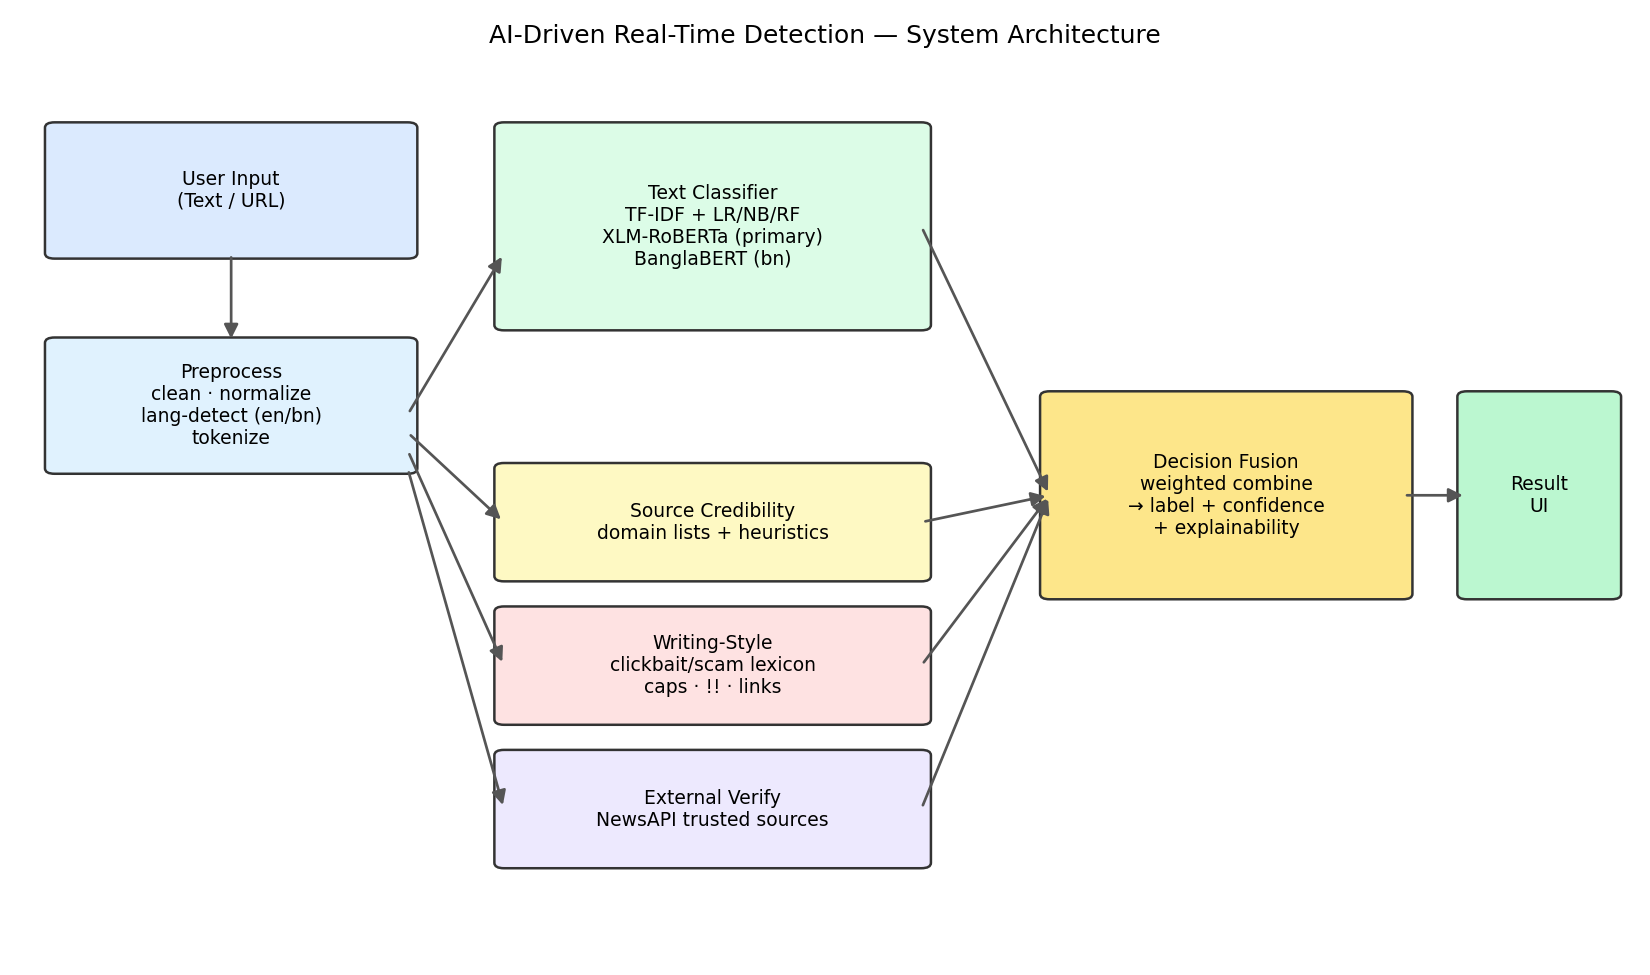
\includegraphics[width=\linewidth]{reports/architecture.png}
  \caption{System architecture. Input text or URL is preprocessed, scored by the
  classifier and the three auxiliary modules, and combined by the decision-fusion
  layer into a final label, confidence score, and explanation.}
  \label{fig:architecture}
\end{figure}

\section{System Model and Assumptions}
\label{sec:assumptions}
The system accepts a single document at a time, supplied either as raw text or as
a URL from which the article body is extracted. Each document is classified into
one of three mutually exclusive classes: \textbf{real}, \textbf{fake}, or
\textbf{malicious}. The following assumptions are made:
\begin{itemize}
  \item \textbf{Textual focus.} Detection is performed on the textual modality.
        Images, audio, and video are out of scope for this version.
  \item \textbf{Language.} Input is English, Bangla, or a mixture; language is
        auto-detected to route normalization.
  \item \textbf{Label availability.} No single public dataset contains all three
        classes, so the corpus is assembled by merging fake-news datasets
        (\emph{real}/\emph{fake}) with phishing and spam datasets (\emph{malicious}).
  \item \textbf{Source signal.} When a URL is available, its domain carries a
        credibility signal; when absent, the credibility module abstains and its
        weight is redistributed.
  \item \textbf{External availability.} External verification depends on a
        third-party news API; the system must degrade gracefully when it is
        unavailable.
\end{itemize}

\section{Proposed Method}
\label{sec:method}

\subsection{Data Collection and Corpus Construction}
The three-class corpus is built by combining publicly available sources:
\emph{real}/\emph{fake} examples are drawn from English (GonzaloA \emph{fake\_news})
and Bangla (BanFakeNews-derived) news datasets, while \emph{malicious} examples
are drawn from SMS-spam and phishing-text datasets. All sources are mapped to a
common schema \texttt{(text, label, lang, source)}. Table~\ref{tab:dataset}
summarizes the class--language distribution of the assembled corpus. The corpus
is split into stratified training, validation, and test partitions (70/15/15).

\begin{table}[t]
  \centering
  \caption{Assembled three-class corpus (class $\times$ language). The full
  statistics are generated in \texttt{reports/dataset\_stats.md}.}
  \label{tab:dataset}
  \begin{tabular}{lrrr}
    \hline
    \textbf{Class} & \textbf{English} & \textbf{Bangla} & \textbf{Total} \\
    \hline
    Real      & 13{,}099 & 576 & 13{,}675 \\
    Fake      & 11{,}119 & 117 & 11{,}236 \\
    Malicious &  7{,}552 &   0 &  7{,}552 \\
    \hline
    \textbf{Total} & 31{,}770 & 693 & 32{,}463 \\
    \hline
  \end{tabular}
\end{table}

\subsection{Preprocessing}
Every document passes through a shared cleaning routine used at both training and
inference time to avoid train--serve skew: Unicode normalization (NFKC, with
Bangla-specific normalization where available), HTML and URL stripping, removal
of non-informative symbols while retaining style-bearing punctuation, whitespace
collapsing, and length truncation. Language is detected from the proportion of
Bengali-script characters and recorded for analysis and routing.

\subsection{Feature Extraction}
Two complementary representations are used. \textbf{TF--IDF} features combine
word $n$-grams ($1$--$2$) and character $n$-grams ($3$--$5$); character $n$-grams
add robustness for Bangla and for the noisy, short text typical of phishing and
spam. \textbf{Contextual embeddings} are produced by a transformer
(Section~\ref{sec:transformer}), capturing meaning and long-range dependencies
that bag-of-features models cannot.

\subsection{Classification Models}
Three classical models are trained on the TF--IDF features as baselines:
\emph{Logistic Regression}, \emph{Multinomial Naive Bayes}, and \emph{Random
Forest}. Class imbalance is handled with balanced class weights. These baselines
are fast, interpretable, and serve as the comparison point for the transformer.

\subsubsection{Transformer Model}
\label{sec:transformer}
The primary model is \textbf{XLM-RoBERTa}, a multilingual transformer fine-tuned
on the three-class corpus; a single multilingual model covers both English and
Bangla without a separate language router. \textbf{BanglaBERT} is additionally
fine-tuned for a Bangla-specific comparison. Fine-tuning uses a maximum sequence
length of 256, a learning rate of $2\times10^{-5}$, and three epochs, selecting
the checkpoint with the best validation macro-F1.

\subsection{Auxiliary Analysis Modules}
\begin{description}
  \item[Source Credibility.] Given a URL, the domain is matched against curated
        trusted and untrusted lists and scored with heuristics (raw-IP hosts,
        abused TLDs, excessive hyphenation, and security-mimicking tokens such as
        \texttt{secure}/\texttt{login}/\texttt{verify}). The output is a risk
        score in $[0,1]$ with a rationale.
  \item[Writing-Style and Behavioral Analysis.] A rule-based analyzer detects
        clickbait, sensational, and scam/phishing phrases (English and Bangla)
        together with surface signals---ALL-CAPS ratio, exclamation runs, and
        link count---returning a suspicion score and the matched spans for
        highlighting.
  \item[External Verification.] Salient keywords are extracted and queried
        against trusted news outlets through a news API; corroboration by
        reputable sources lowers risk, while absence is treated as neutral rather
        than as proof of falsity. The module is cached and timeout-guarded.
\end{description}

\subsection{Decision Fusion and Explainability}
\label{sec:fusion}
Each module emits a risk score in $[0,1]$ (higher $=$ more likely
fake/malicious); the classifier contributes $1-P(\text{real})$. The fused risk is
a weighted average of the available module risks; unavailable modules (e.g., no
URL, no API key) are removed and their weight is renormalized across the rest. If
the fused risk is below a threshold the document is labelled \emph{real};
otherwise the \emph{fake}-versus-\emph{malicious} decision follows the
classifier's relative class probabilities, nudged toward \emph{malicious} when
strong phishing-style signals are present. The confidence score combines the
fused risk with the classifier's decision margin. For explainability the system
returns each module's weighted contribution and reasons, the classifier's class
probabilities, and the highlighted style spans.

\subsection{Any Secondary Contribution}
Beyond the unified three-class detector, a secondary contribution is the
\emph{graceful-degradation fusion} scheme: the pipeline produces a calibrated,
explained decision even when external signals (URL, news API) are missing, by
dynamically redistributing fusion weights---making the system practical for
real-world deployment where such signals are frequently unavailable.

\subsection{Discussion}
The modular design separates concerns: the classifier captures linguistic
content, while the auxiliary modules contribute orthogonal signals (provenance,
manipulation cues, and external corroboration). This both improves robustness and
yields transparent, per-factor explanations, addressing the trust and
interpretability gaps identified in Chapter~\ref{ch:methodology}'s motivation.

\section{Conclusion}
This chapter described the proposed bilingual, multi-module detection system: its
data construction, preprocessing, feature extraction, classical and transformer
classifiers, auxiliary analyzers, and the decision-fusion layer that unifies them
into an explainable real-time prediction. The next chapter evaluates the system.
